% TO-DO:
% * slides to mention big achievements, 附件

\documentclass[16pt]{beamer}

\ifdefined\chinchin
\usepackage[CJKspace]{xeCJK}
%\setCJKmainfont[BoldFont=SimHei,ItalicFont=AR PL KaitiM GB]{Alibaba PuHuiTi}
\setCJKmainfont{Alibaba PuHuiTi}
\newcommand{\cc}[2]{#1}
\else
\newcommand{\cc}[2]{#2}
\renewcommand{\baselinestretch}{0.8} 
\fi

%\usepackage{newtxtext,newtxmath}	% use Times Roman font
%\usepackage{newtxtext}
%\renewcommand{\familydefault}{\sfdefault}
\usefonttheme{serif}
\usefonttheme{professionalfonts}
%\setbeamertemplate{theorems}[numbered]
\setbeamertemplate{caption}{\insertcaption} 	% no `Figure' prefix before caption

\mode<presentation> {

%\usetheme{default}
%\usetheme{AnnArbor}
%\usetheme{Antibes}
%\usetheme{Bergen}
%\usetheme{Berkeley}
%\usetheme{Berlin}
%\usetheme{Boadilla}
%\usetheme{CambridgeUS}
%\usetheme{Copenhagen}
%\usetheme{Darmstadt}
%\usetheme{Dresden}
%\usetheme{Frankfurt}
%\usetheme{Goettingen}
%\usetheme{Hannover}
%\usetheme{Ilmenau}
%\usetheme{JuanLesPins}
%\usetheme{Luebeck}
\usetheme{Madrid}
%\usetheme{Malmoe}
%\usetheme{Marburg}
%\usetheme{Montpellier}
%\usetheme{PaloAlto}
%\usetheme{Pittsburgh}
%\usetheme{Rochester}
%\usetheme{Singapore}
%\usetheme{Szeged}
%\usetheme{Warsaw}

%\usecolortheme{albatross}
%\usecolortheme{beaver}
%\usecolortheme{beetle}
%\usecolortheme{crane}
%\usecolortheme{dolphin}
%\usecolortheme{dove}
%\usecolortheme{fly}
%\usecolortheme{lily}
\usecolortheme{orchid}
%\usecolortheme{rose}
%\usecolortheme{seagull}
%\usecolortheme{seahorse}
%\usecolortheme{whale}
%\usecolortheme{wolverine}		% Hofstra

%\setbeamertemplate{footline} % To remove the footer line in all slides uncomment this line
\setbeamertemplate{footline}[page number] % To replace the footer line in all slides with a simple slide count uncomment this line
\setbeamertemplate{navigation symbols}{} % To remove the navigation symbols from the bottom of all slides uncomment this line
}

\setbeamertemplate{headline}{}
\setbeamersize{text margin left=1mm,text margin right=1mm} 
\settowidth{\leftmargini}{\usebeamertemplate{itemize item}}
\addtolength{\leftmargini}{\labelsep}

\usepackage[backend=biber,style=numeric]{biblatex}
\bibliography{../AGI-book}
% \renewcommand*{\bibfont}{\footnotesize}
\setbeamertemplate{bibliography item}[text]

\usepackage{graphicx} % Allows including images
\usepackage{tikz-cd}
\usepackage{tikz}
\usepackage[export]{adjustbox}% http://ctan.org/pkg/adjustbox
\usepackage{verbatim} % comments
% \usepackage{tikz-cd}  % commutative diagrams
% \newcommand{\tikzmark}[1]{\tikz[overlay,remember picture] \node (#1) {};}
% \usepackage{booktabs} % Allows the use of \toprule, \midrule and \bottomrule in tables
% \usepackage{amssymb}  % \leftrightharpoons
% \usepackage{wasysym} % frownie face
% \usepackage{newtxtext,newtxmath}	% Times New Roman font
% \usepackage{sansmath}

\newcommand{\emp}[1]{\textbf{\color{violet}#1}}
\newcommand{\vect}[1]{\boldsymbol{#1}}
\newcommand{\tab}{\hspace*{1cm}}
\newcommand*\confoundFace{$\vcenter{\hbox{\includegraphics[scale=0.2]{../confounded-face.jpg}}}$}
\newcommand{\smiley}{$\vcenter{\hbox{\includegraphics[scale=0.05]{../smiling-face.png}}}$}

\makeatletter
\renewcommand{\boxed}[1]{\fbox{\m@th$\displaystyle\scalebox{0.9}{#1}$} \,}
\makeatother

%%%%%%%% Make table of contents %%%%%%%

\newif\ifframeinlbf
\frameinlbftrue
\makeatletter
\newcommand\listofframes{\@starttoc{lbf}}
\makeatother
\addtobeamertemplate{frametitle}{}{%
	\ifframeinlbf
	\addcontentsline{lbf}{section}{\protect\makebox[2em][l]{%
			\protect\usebeamercolor[fg]{structure}\insertframenumber\hfill}%
		\insertframetitle\par}%
	\else\fi
}

%%%%%%%% Include Parts in TOC %%%%%%%

\makeatletter
\AtBeginPart{%
	\addtocontents{toc}{\protect\beamer@partintoc{\the\c@part}{\beamer@partnameshort}{\the\c@page}}%
}
%% number, shortname, page.
\providecommand\beamer@partintoc[3]{%
	\ifnum\c@tocdepth=-1\relax
	% requesting onlyparts.
	\makebox[6em]{PART #1:} #2
	\par
	\fi
}
\define@key{beamertoc}{onlyparts}[]{%
	\c@tocdepth=-1\relax
}
\makeatother%

%----------------------------------------------------------------------------------------
%	TITLE PAGE
%----------------------------------------------------------------------------------------

\title[AGI via Logic]{{\Huge AGI via Combining Logic and Deep Learning}
 \\ \vspace*{0.4cm} AGI 2021 Conference}
\author{\cc{YKY}{YKY}} % Your name
%\institute[] % Your institution as it will appear on the bottom of every slide, may be shorthand to save space
%{
%Independent researcher, Hong Kong \\ % Your institution for the title page
%\medskip
%\textit{generic.intelligence@gmail.com} % Your email address
%}
\date{\today} % Date, can be changed to a custom date

\begin{document}

\frameinlbffalse
\addtocounter{page}{-1}
\begin{frame}[plain,noframenumbering]
\titlepage
\end{frame}

\addtocounter{page}{-1}
\begin{frame}[noframenumbering]
\frametitle{Table of contents}
\listofframes
% \vspace*{0.5cm}
% 多谢 支持 \smiley
\end{frame}

%----------------------------------------------------------------------------------------
%	PRESENTATION SLIDES
%----------------------------------------------------------------------------------------

%------------------------------------------------

\frameinlbftrue

\part{BERT / GPT}
\frame{\partpage}

\begin{frame}
\frametitle{BERT is AGI}
\begin{itemize}
	\item BERT can generate texts, answer questions, and even write code
	\item BERT has learned human knowledge from text corpora
	\item Therefore, BERT is approximately AGI
	\item BERT also demonstrates that our computing power is \\
			 in the \textbf{ballpark} of AGI
	\item I predict that human-level AGI will emerge within 5-6 years
\end{itemize}
\end{frame}

\begin{frame}
\frametitle{Equivariance of the Transformer}
\begin{itemize}
	\item Many people already know this: \\
	the Transformer module is \textbf{equivariant} in its inputs and outputs:
\end{itemize}
\centering
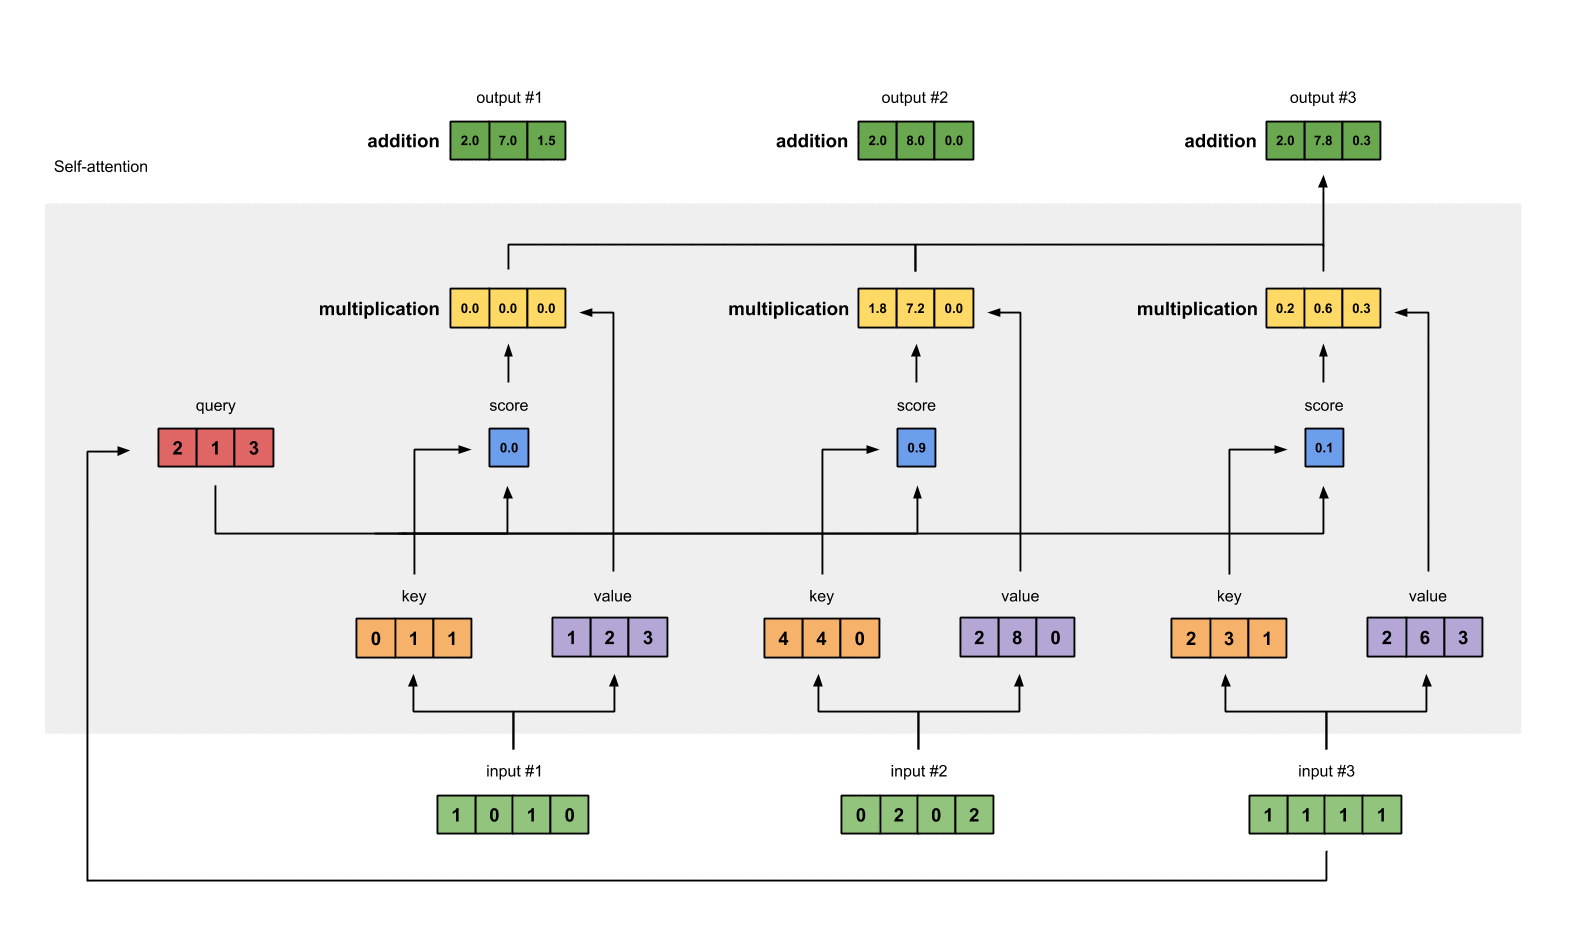
\includegraphics[scale=0.2]{self-attention.png}
\end{frame}

\begin{frame}
\frametitle{BERT's Hidden Representation}
\begin{itemize}
	\item A simplified view of how BERT performs \textbf{question-answering} or \textbf{logic deduction}:
\end{itemize}
\vspace*{1em}
\centering
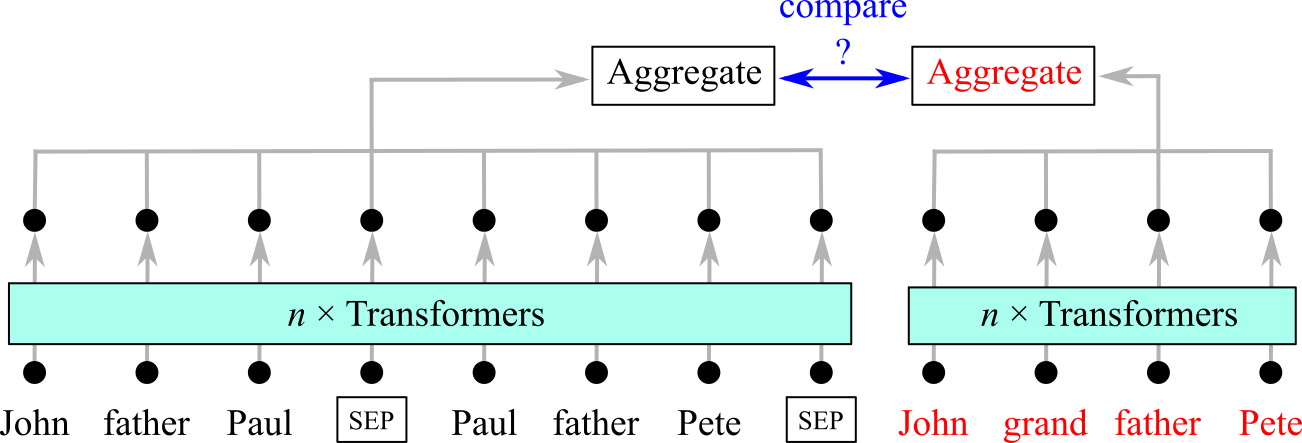
\includegraphics[scale=0.7]{Transformer-QnA.png}
\end{frame}

\begin{frame}
\frametitle{BERT compared with AGI architecture}
\begin{itemize}
	\item A minimal AGI architecture is like this:
	\begin{equation}
	\vcenter{\hbox{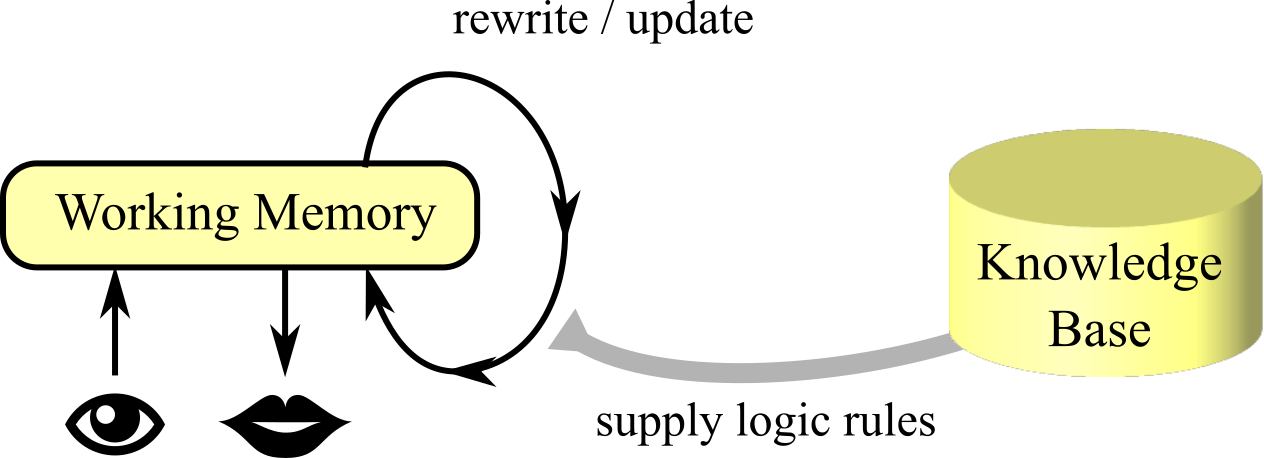
\includegraphics[scale=0.5]{LBAI-architecture.png}}}
	\end{equation}
\end{itemize}
\end{frame}

\begin{frame}
\frametitle{AGI as Sequence-to-sequence Rewriter}
\begin{itemize}
	\item The \textbf{state} of a logic system is a \textbf{set} of propositions
	\item So state = sequence of sequences, \\
		The 2nd level represents predicates and terms \textbf{inside} a proposition
	\begin{equation}
	\vcenter{\hbox{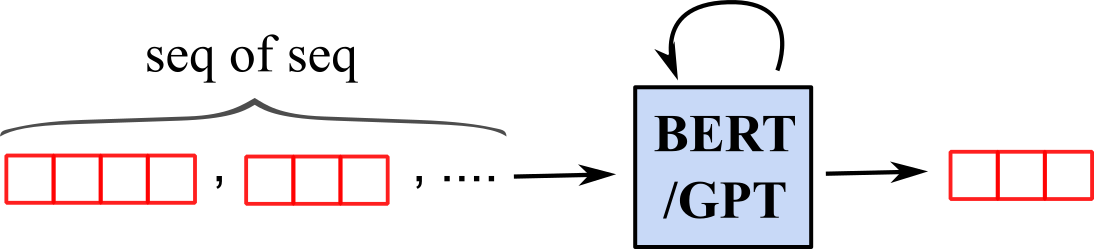
\includegraphics[scale=0.5]{seq-seq-2-seq-with-BERT.png}}}
	\end{equation}
\end{itemize}
\end{frame}

\begin{frame}
\frametitle{BERT with Long-Term Memory}
\begin{itemize}
	\item With logic, it is easier to design cognitive architectures, \\
		eg: long-term memory module
\begin{equation}
\vcenter{\hbox{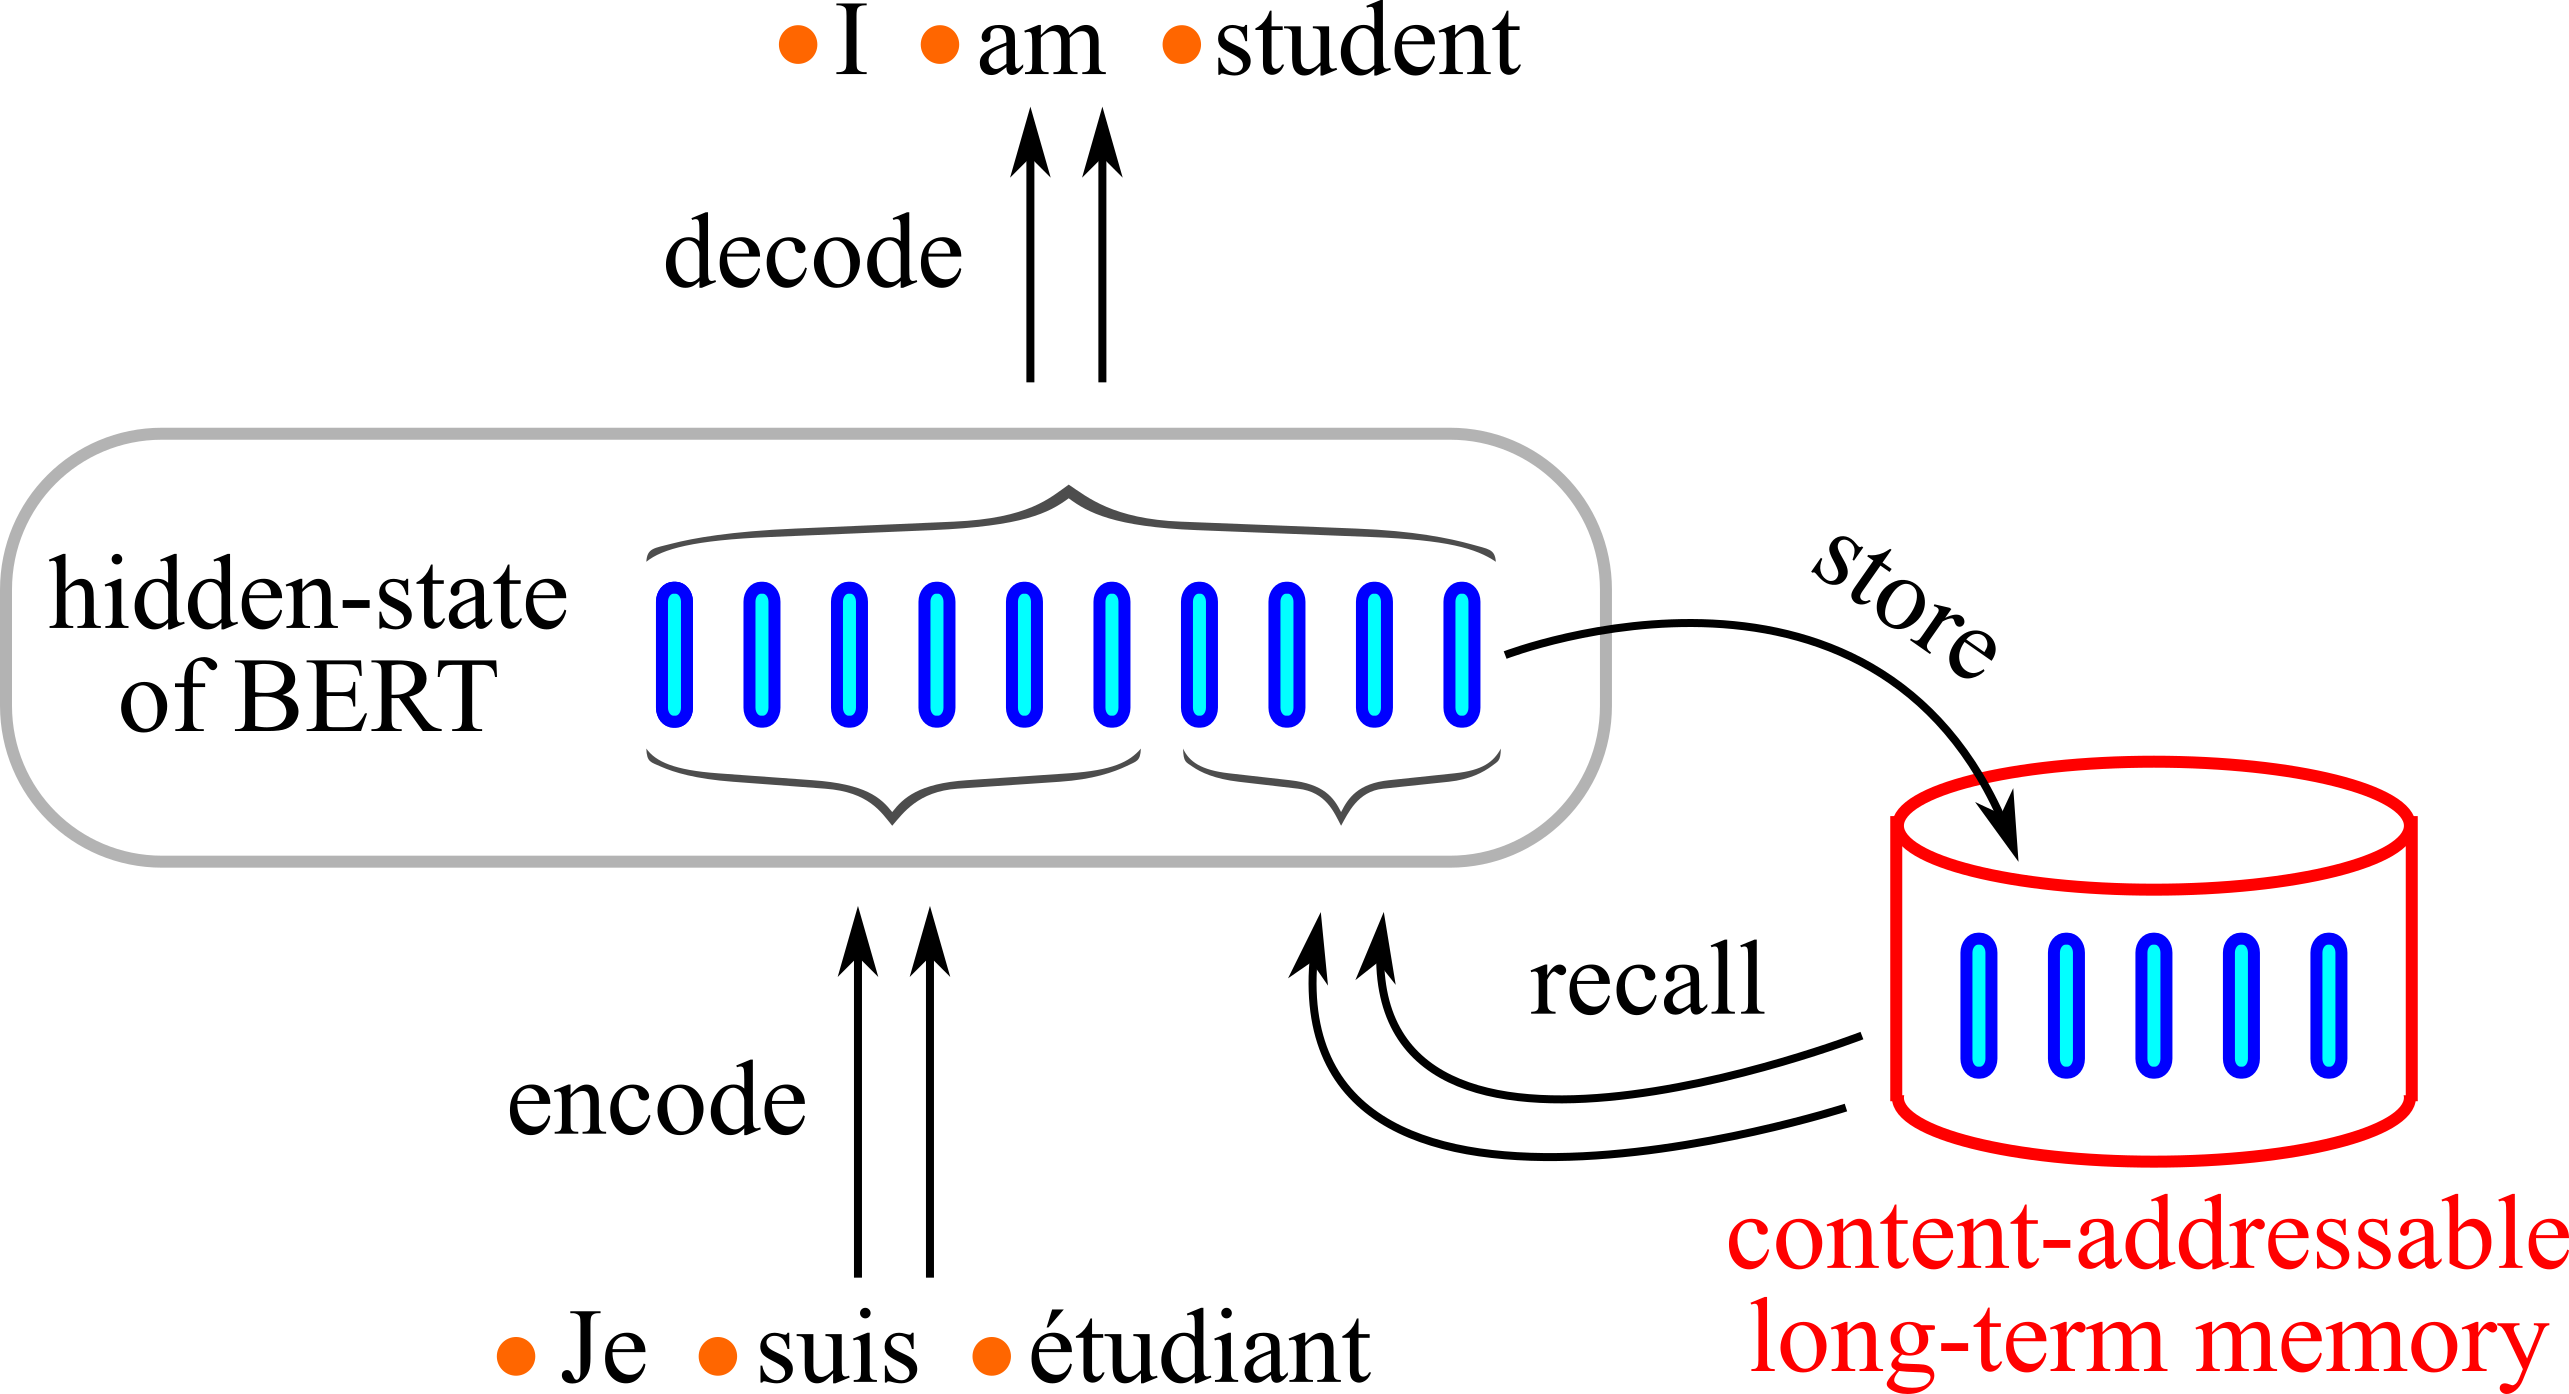
\includegraphics[scale=0.5]{long-term-memory.png}}}
\end{equation}
\end{itemize}
\end{frame}

\begin{frame}
\frametitle{Additivity of Word Embeddings}
\begin{itemize}
	\item The sine waves are \textbf{Positional Encodings}
	\item We can see that \textbf{Word Embeddings} can co-exist \\
	if embedding dimension is large enough
\end{itemize}
\centering
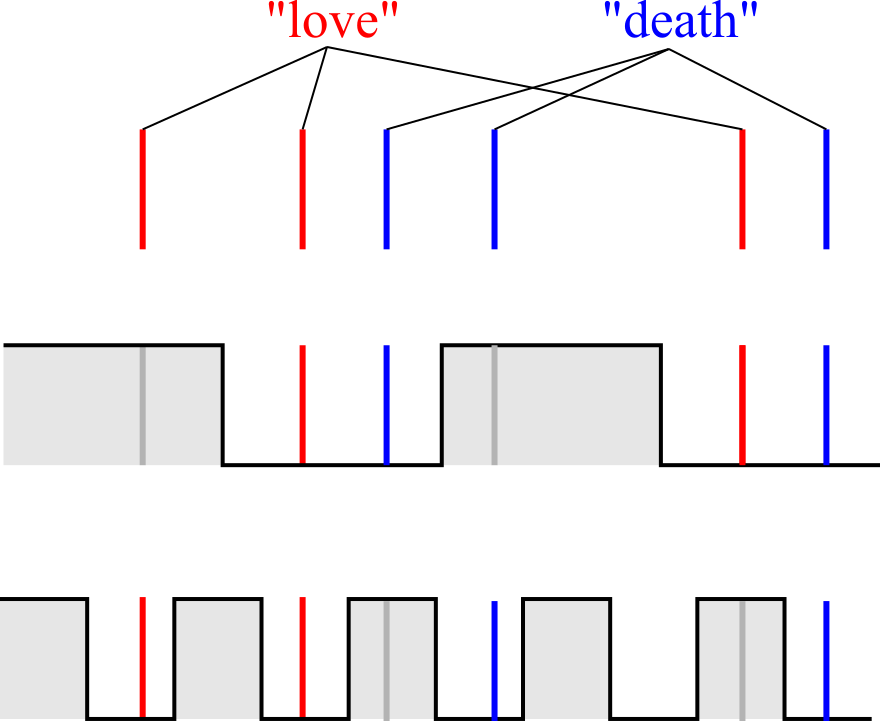
\includegraphics[scale=0.5]{positional-encoding.png}
\vspace*{1em}
\begin{itemize}
	\item This suggests that word embeddings can be added together to give \textbf{composite} meanings
\end{itemize}
\end{frame}

\begin{frame}
\frametitle{Memory Recall}
\begin{itemize}
\item Integrate seamlessly with \emp{knowledge graphs}
\item Graphs are made up of edges, \\
	edges = relations between nodes = propositions:
\begin{equation}
\vcenter{\hbox{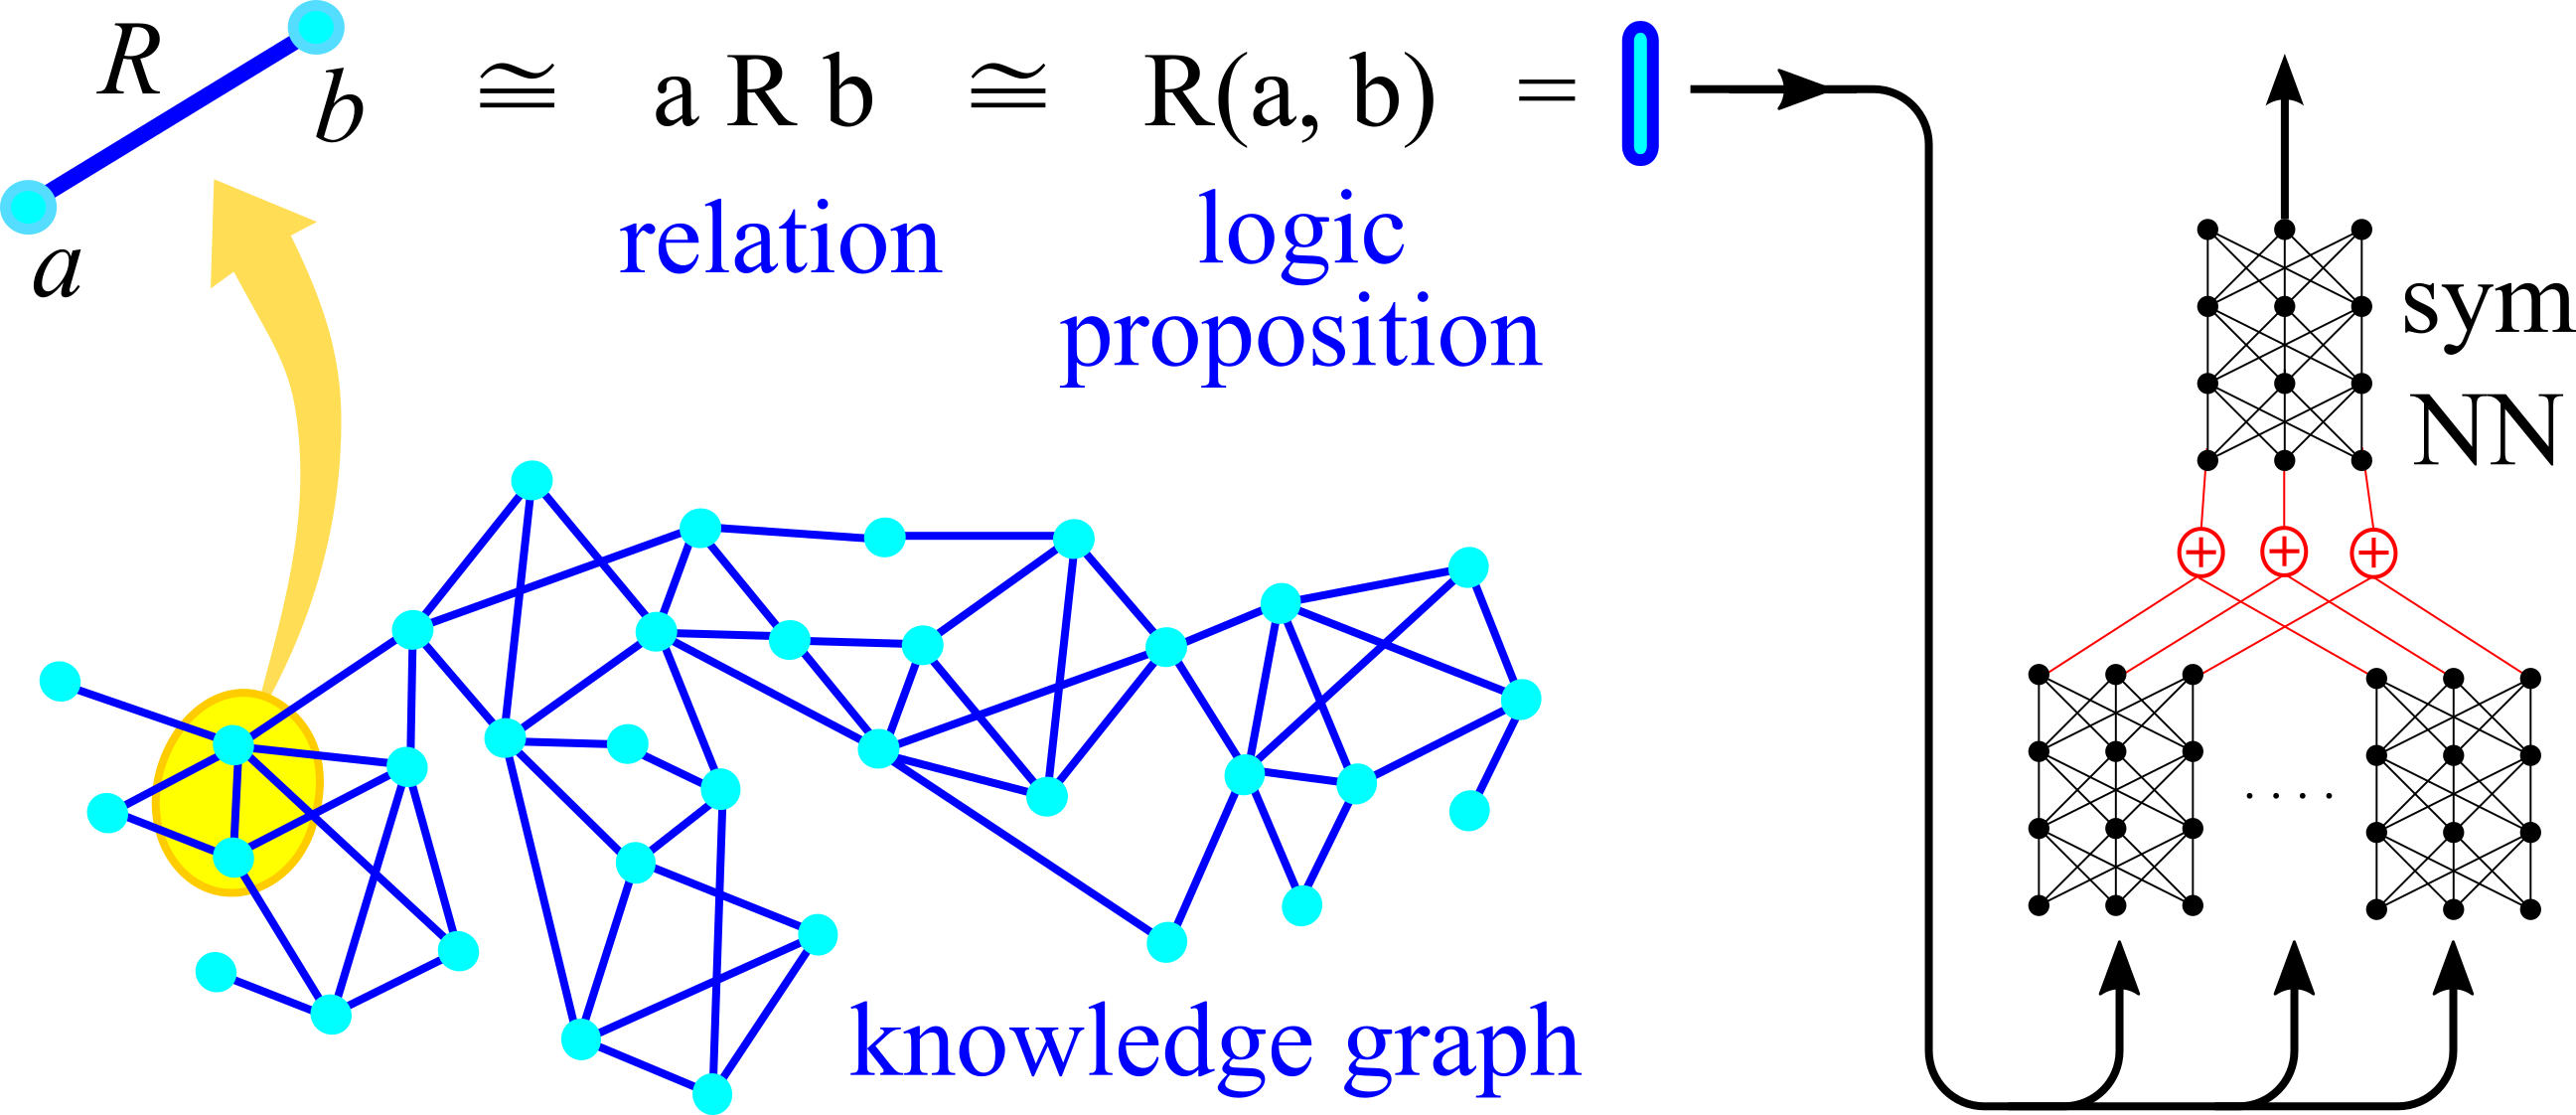
\includegraphics[scale=0.6]{knowledge-graph.png}}}
\end{equation}
\end{itemize}
\end{frame}

\part{Reinforcement Learning}
\frame{\partpage}

\begin{frame}
\frametitle{This is a lamprey}
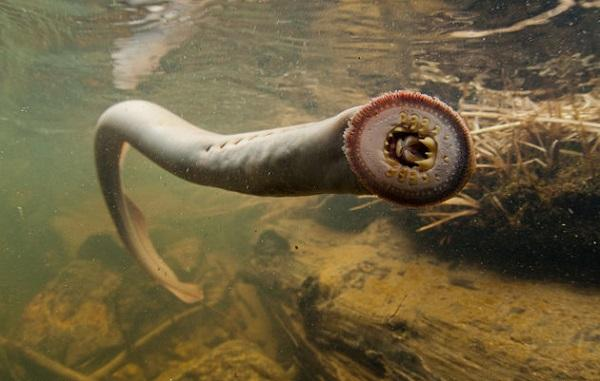
\includegraphics[scale=0.65]{lamprey.jpg}
\end{frame}

\begin{frame}
\frametitle{Evolution of the Neocortex}
\centering
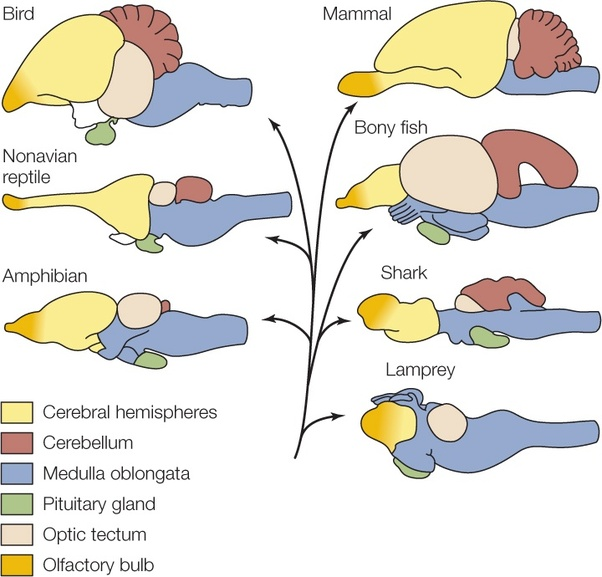
\includegraphics[scale=0.4]{lamprey-to-neocortex.jpg}
\end{frame}

\begin{frame}
\frametitle{Books}
\centering
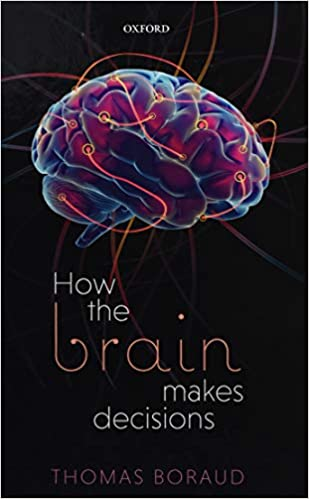
\includegraphics[scale=0.45]{How-the-Brain-Makes-Decisions_(cover).jpg}
\hspace*{2em}
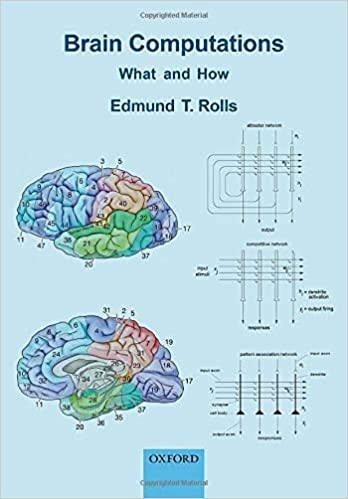
\includegraphics[scale=0.45]{Brain-Computations_(cover).jpg}
\end{frame}

\begin{frame}
\frametitle{How the Basal Ganglia makes Decisions}
\centering
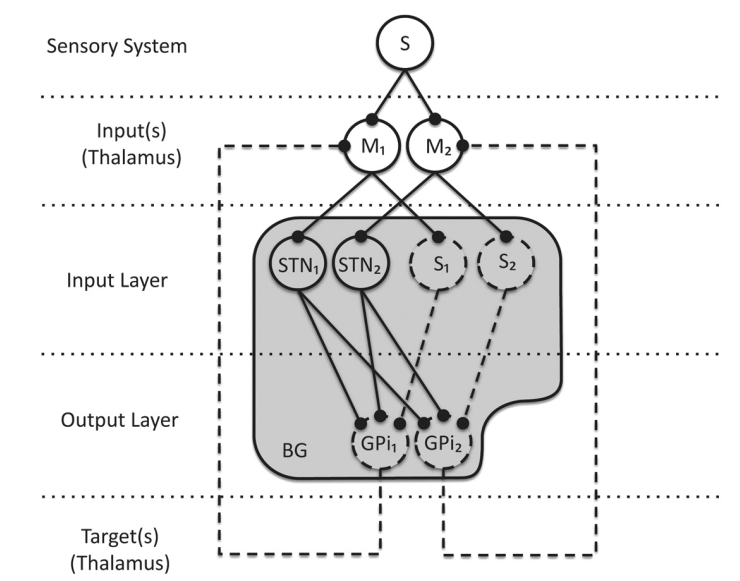
\includegraphics[scale=0.4]{diencephalic-loop.png}
\end{frame}

\begin{frame}
\frametitle{Sub-networks of the Neocortex}
\centering
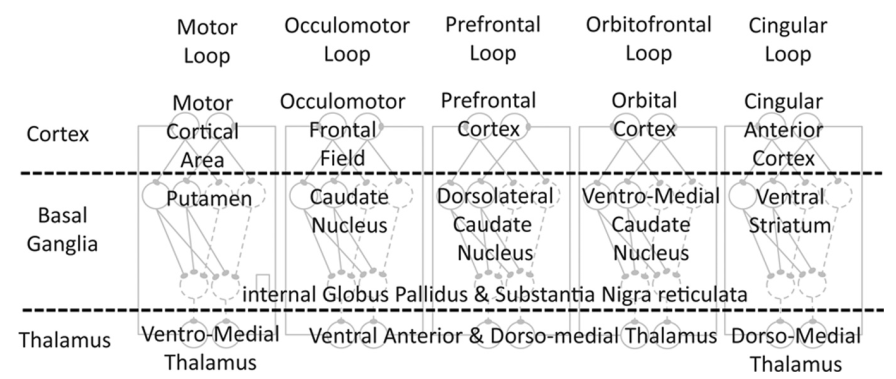
\includegraphics[scale=0.4]{telencephalic-loop.png}
\end{frame}

\begin{frame}
\frametitle{Neocortex vs Reinforcement Learning}
\centering
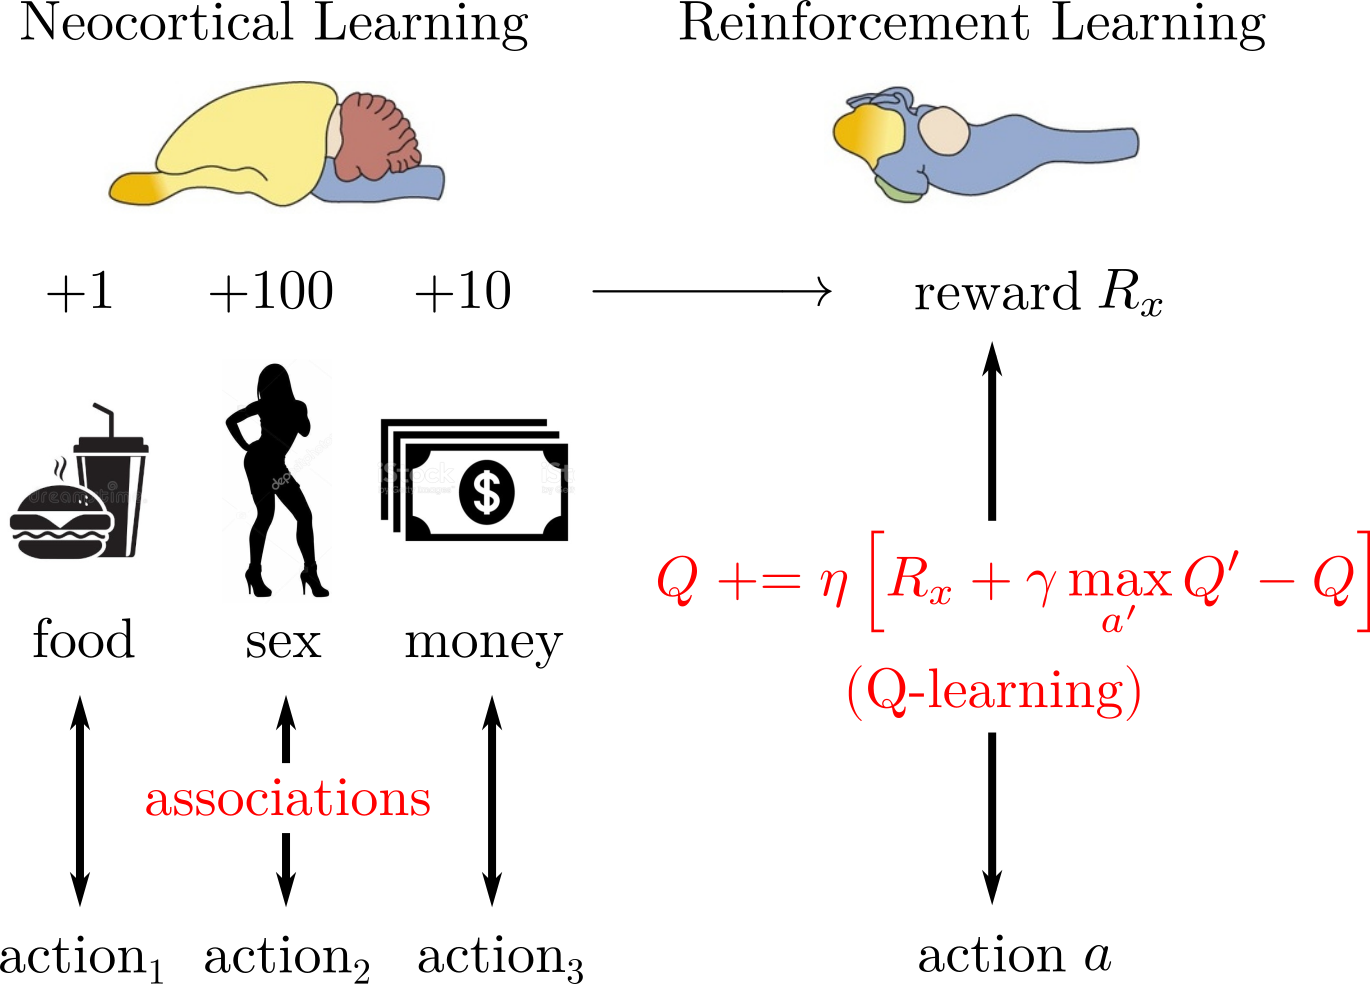
\includegraphics[scale=0.5]{neocortex-vs-RL.png}
\end{frame}

\part{Model-based vs Syntax-based}
\frame{\partpage}

\begin{frame}
\frametitle{What is a Model?}
\centering
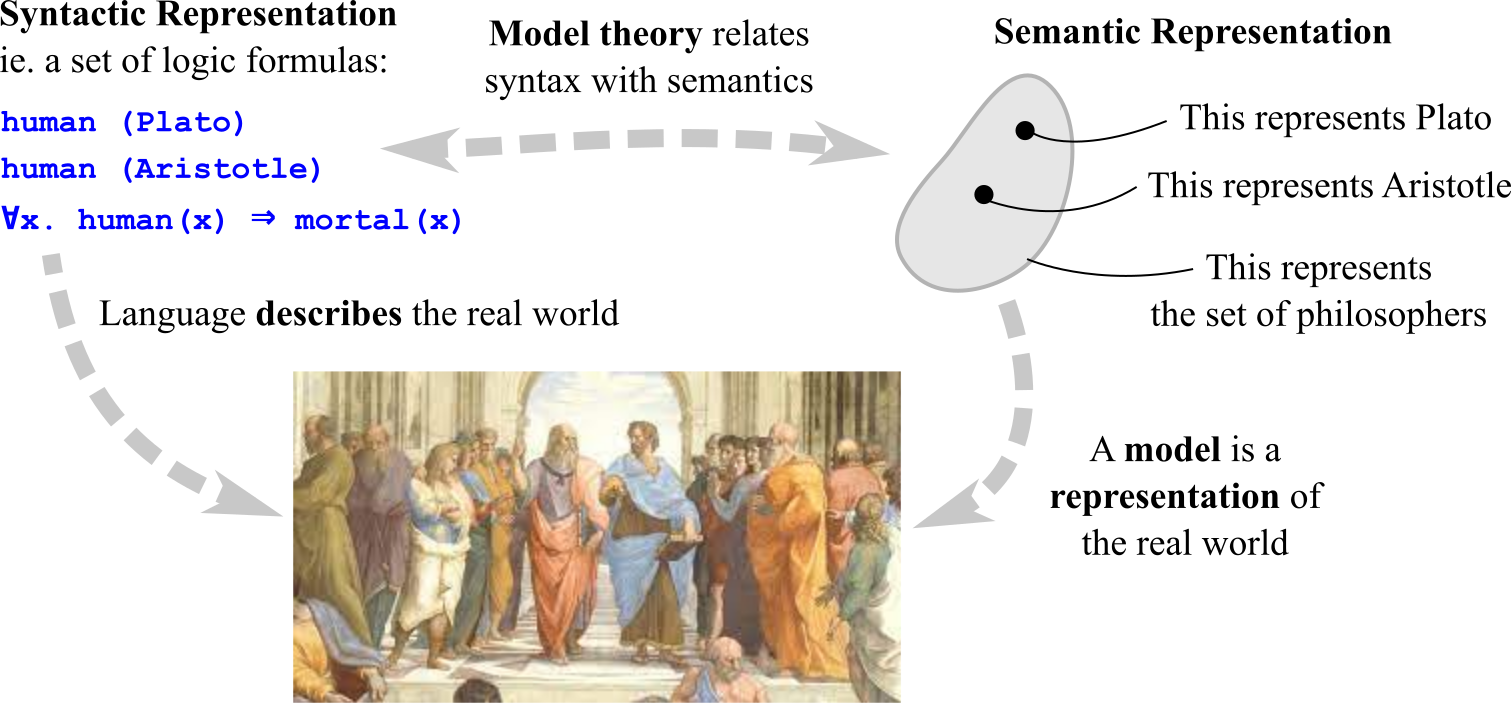
\includegraphics[scale=0.6]{syntax-and-semantics-(cartoon).png}
\end{frame}

\begin{frame}
\frametitle{Hitzler's Core Method}
\begin{itemize}
	\item The \textbf{semantic operator} $\mathcal{T}_P$ updates an interpretation to another interpretation:
\end{itemize}
\centering
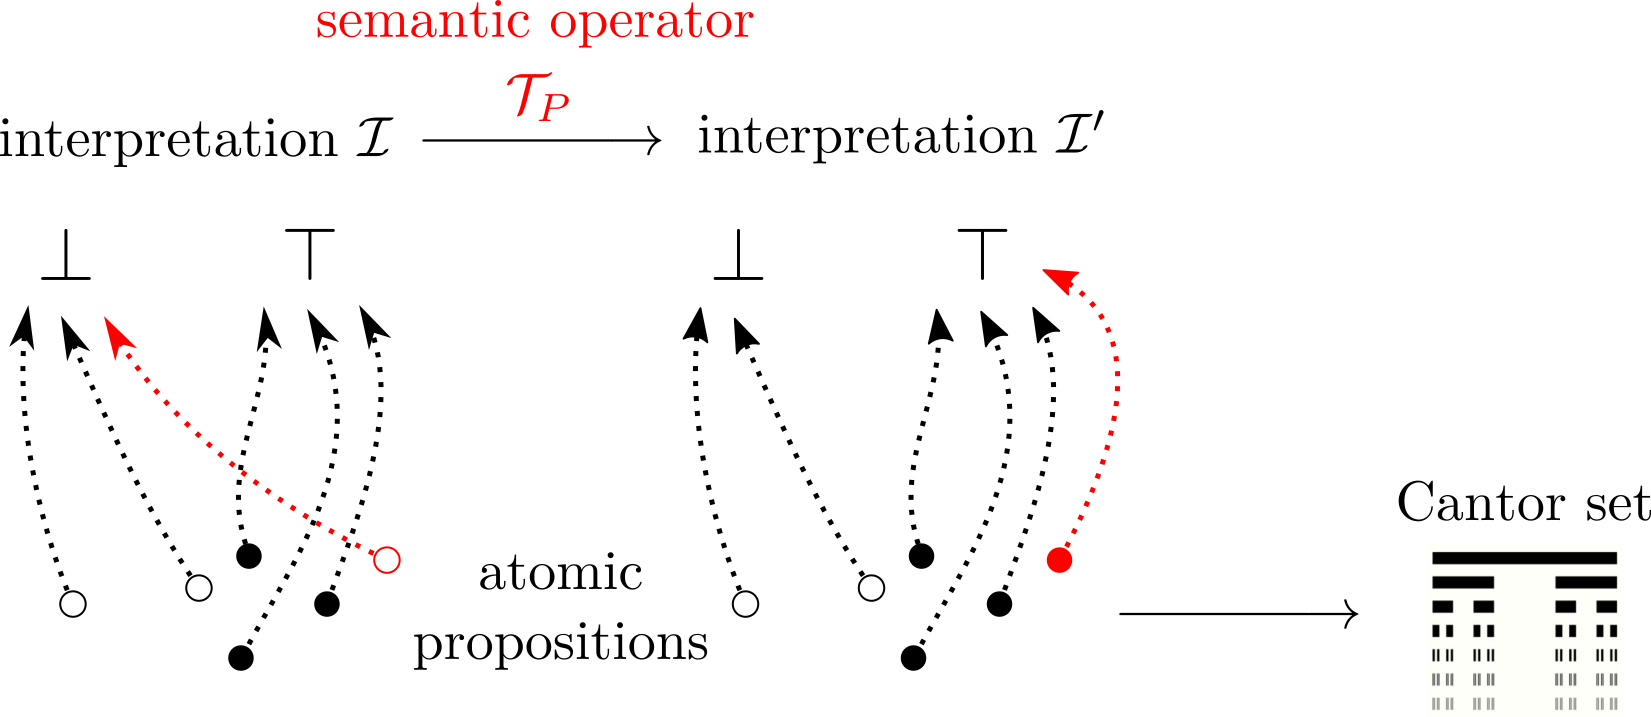
\includegraphics[scale=0.5]{Hitzler-semantic-operator.png}
\end{frame}

\begin{frame}
\frametitle{Hitzler's Core Method}
\begin{itemize}
\item The \textbf{level mapping} $\iota$ takes an interpretation to a real number:
\end{itemize}
\begin{equation}
\vcenter{\hbox{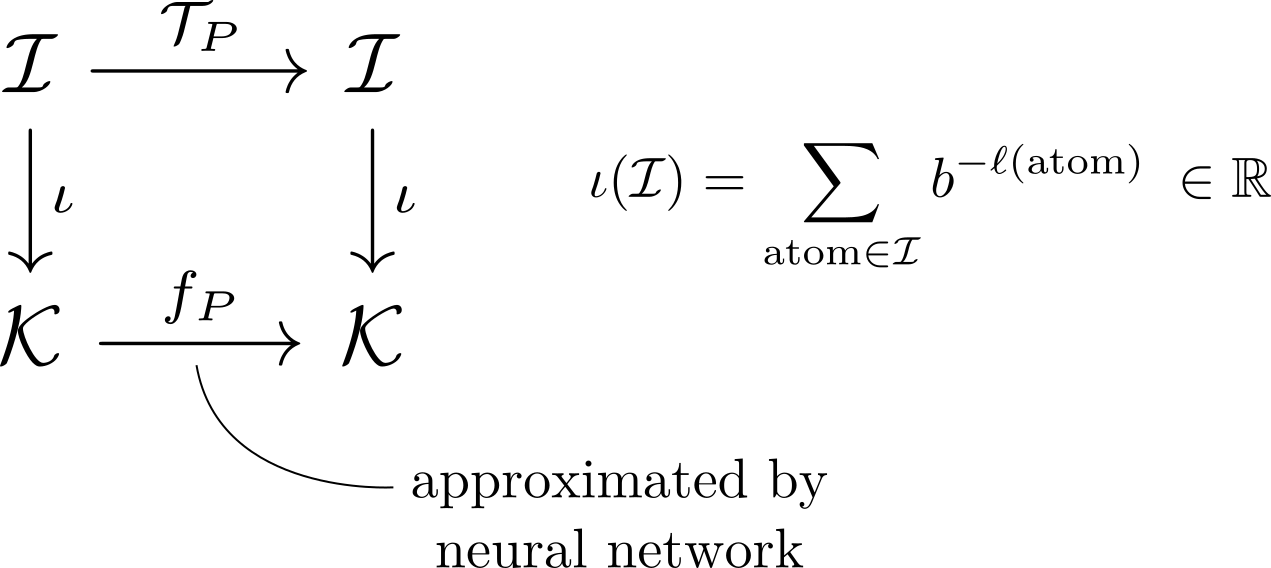
\includegraphics[scale=0.5]{Hitzler-level-mapping.png}}} \nonumber
\end{equation}
\end{frame}

%\part{Categorical Logic}
%\frame{\partpage}

%\begin{frame}
%\frametitle{Categorical Logic}
%\begin{itemize}
%	\item Quantifier as adjunctions
%\end{itemize}
%\end{frame}

\begin{frame}
\frametitle{Fibrations}
\begin{itemize}
	\item ``Floating'' regions and points as models
	\begin{equation}
	\vcenter{\hbox{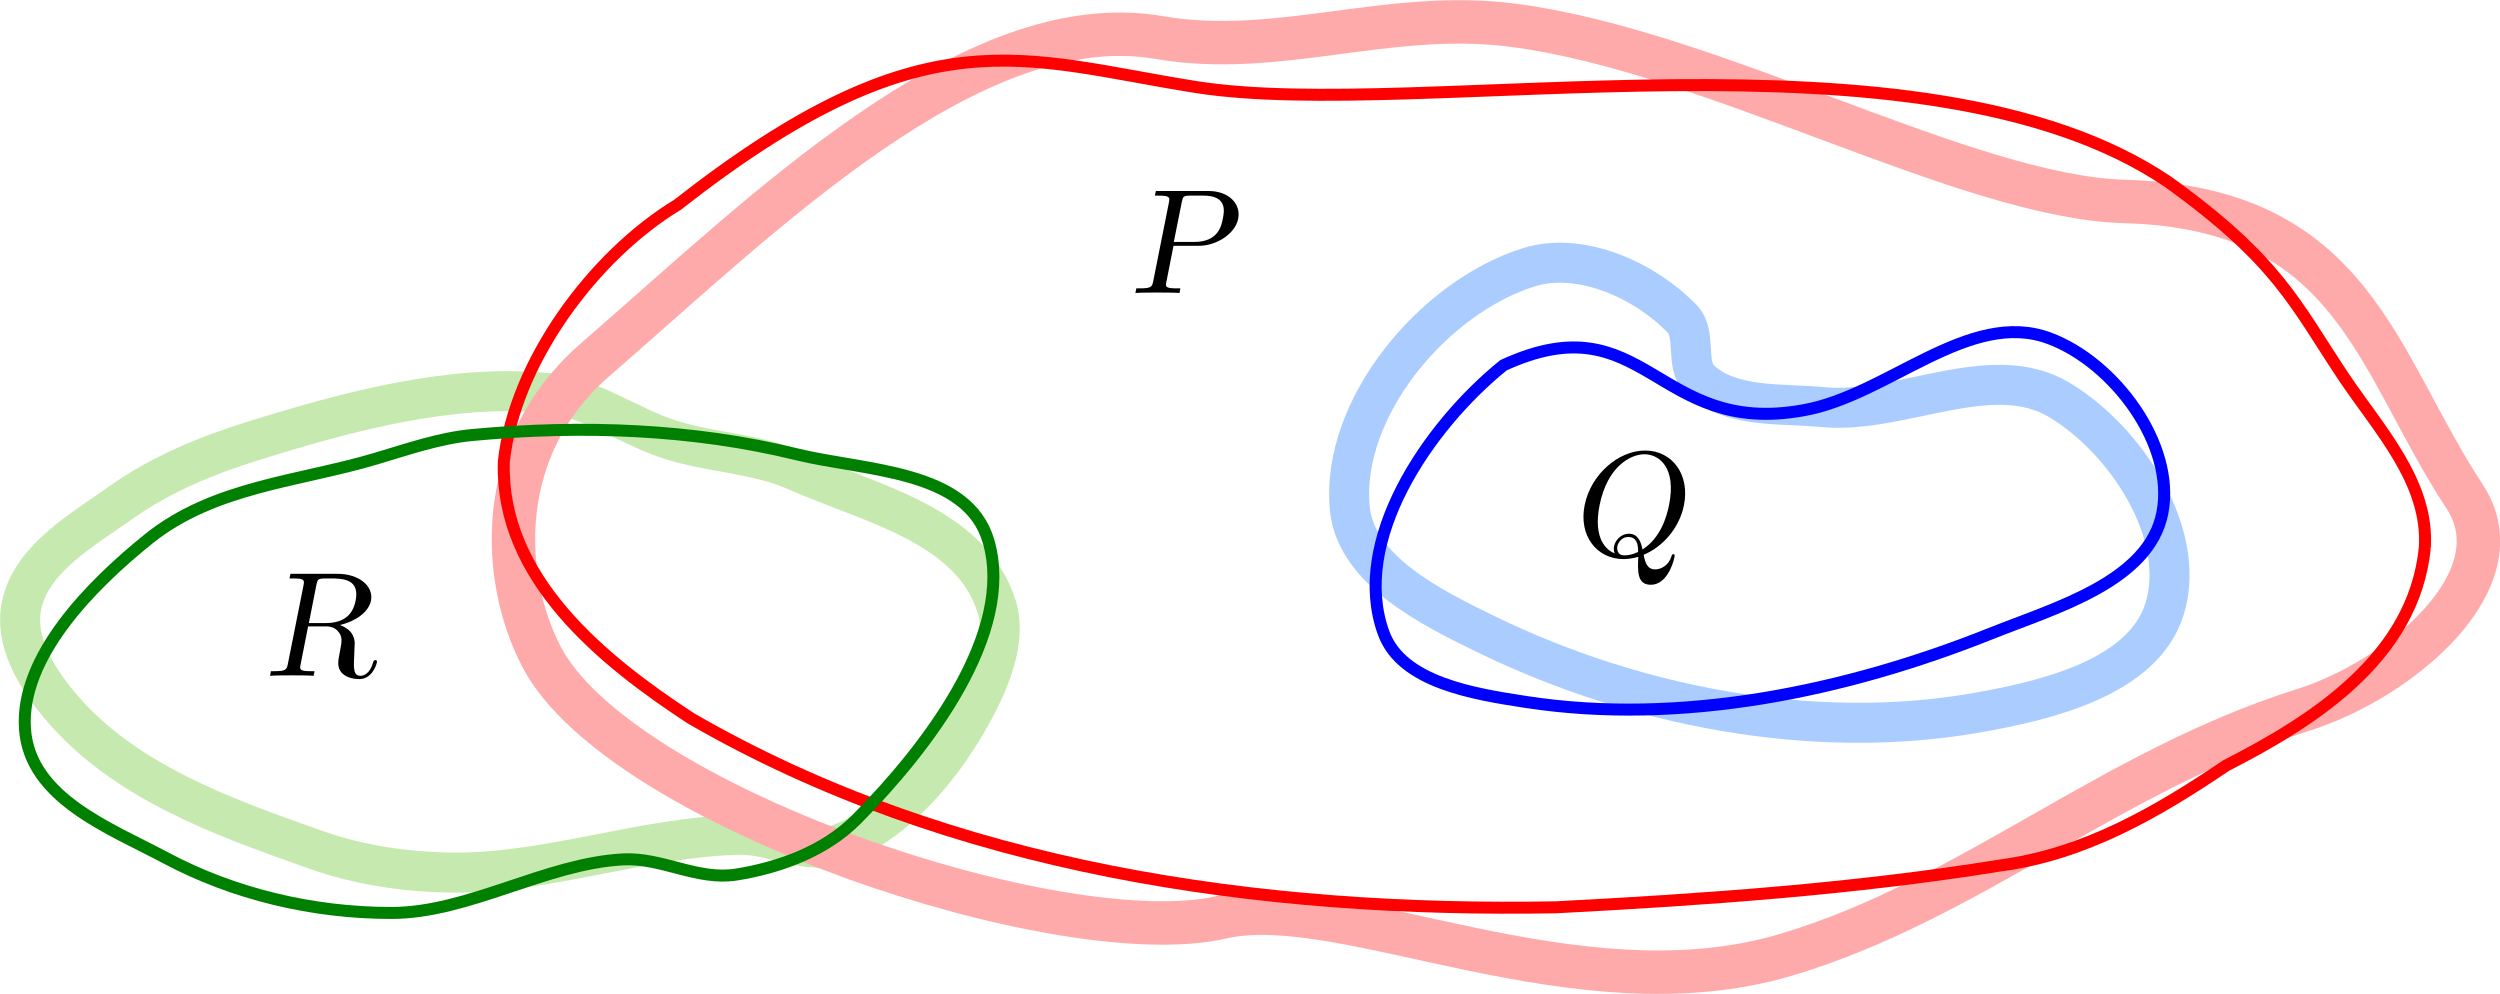
\includegraphics[scale=0.4]{floating-sets-1.png}}}
	\nonumber
	\end{equation}
	\item ``Fibration'' structure of predicates
	\begin{equation}
	\vcenter{\hbox{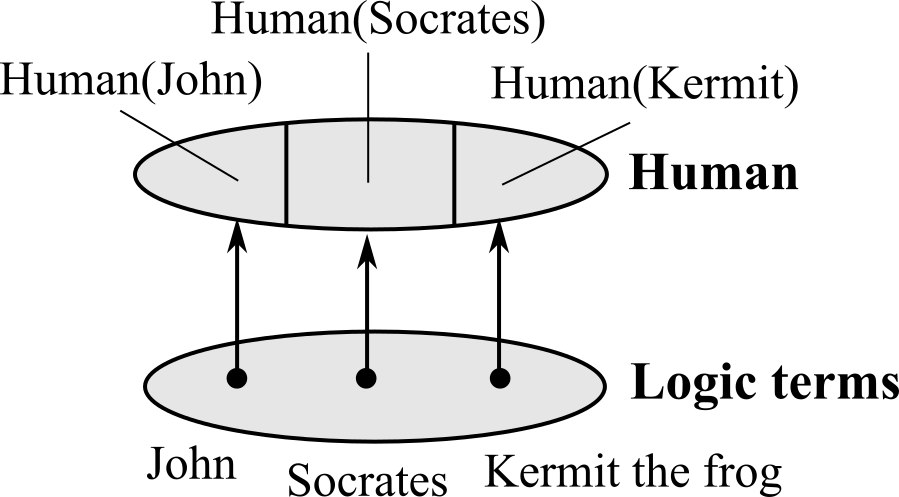
\includegraphics[scale=0.5]{dependent-type.png}}}
	\nonumber
	\end{equation}
\end{itemize}
\end{frame}

\part{No Free Lunch and Inductive Bias}
\frame{\partpage}

\begin{frame}
\frametitle{Symmetry and inductive bias}
\begin{itemize}
	\item \cc{
	在数学上,\emp{对称性} 经常能简化计算,所以数学家 特别喜欢 对称}{
	In mathematics, symmetry often simplifies computation, which is why mathematicians love to study symmetries
	}
	\item \cc{
	在机器学习中,经常要引入 归纳偏好 (inductive bias),缩小 \emp{搜寻空间}:}{
	In machine learning, one introduces \emp{inductive bias} to narrow down the \textbf{search space}:
	}
	\begin{equation}
	\vcenter{\hbox{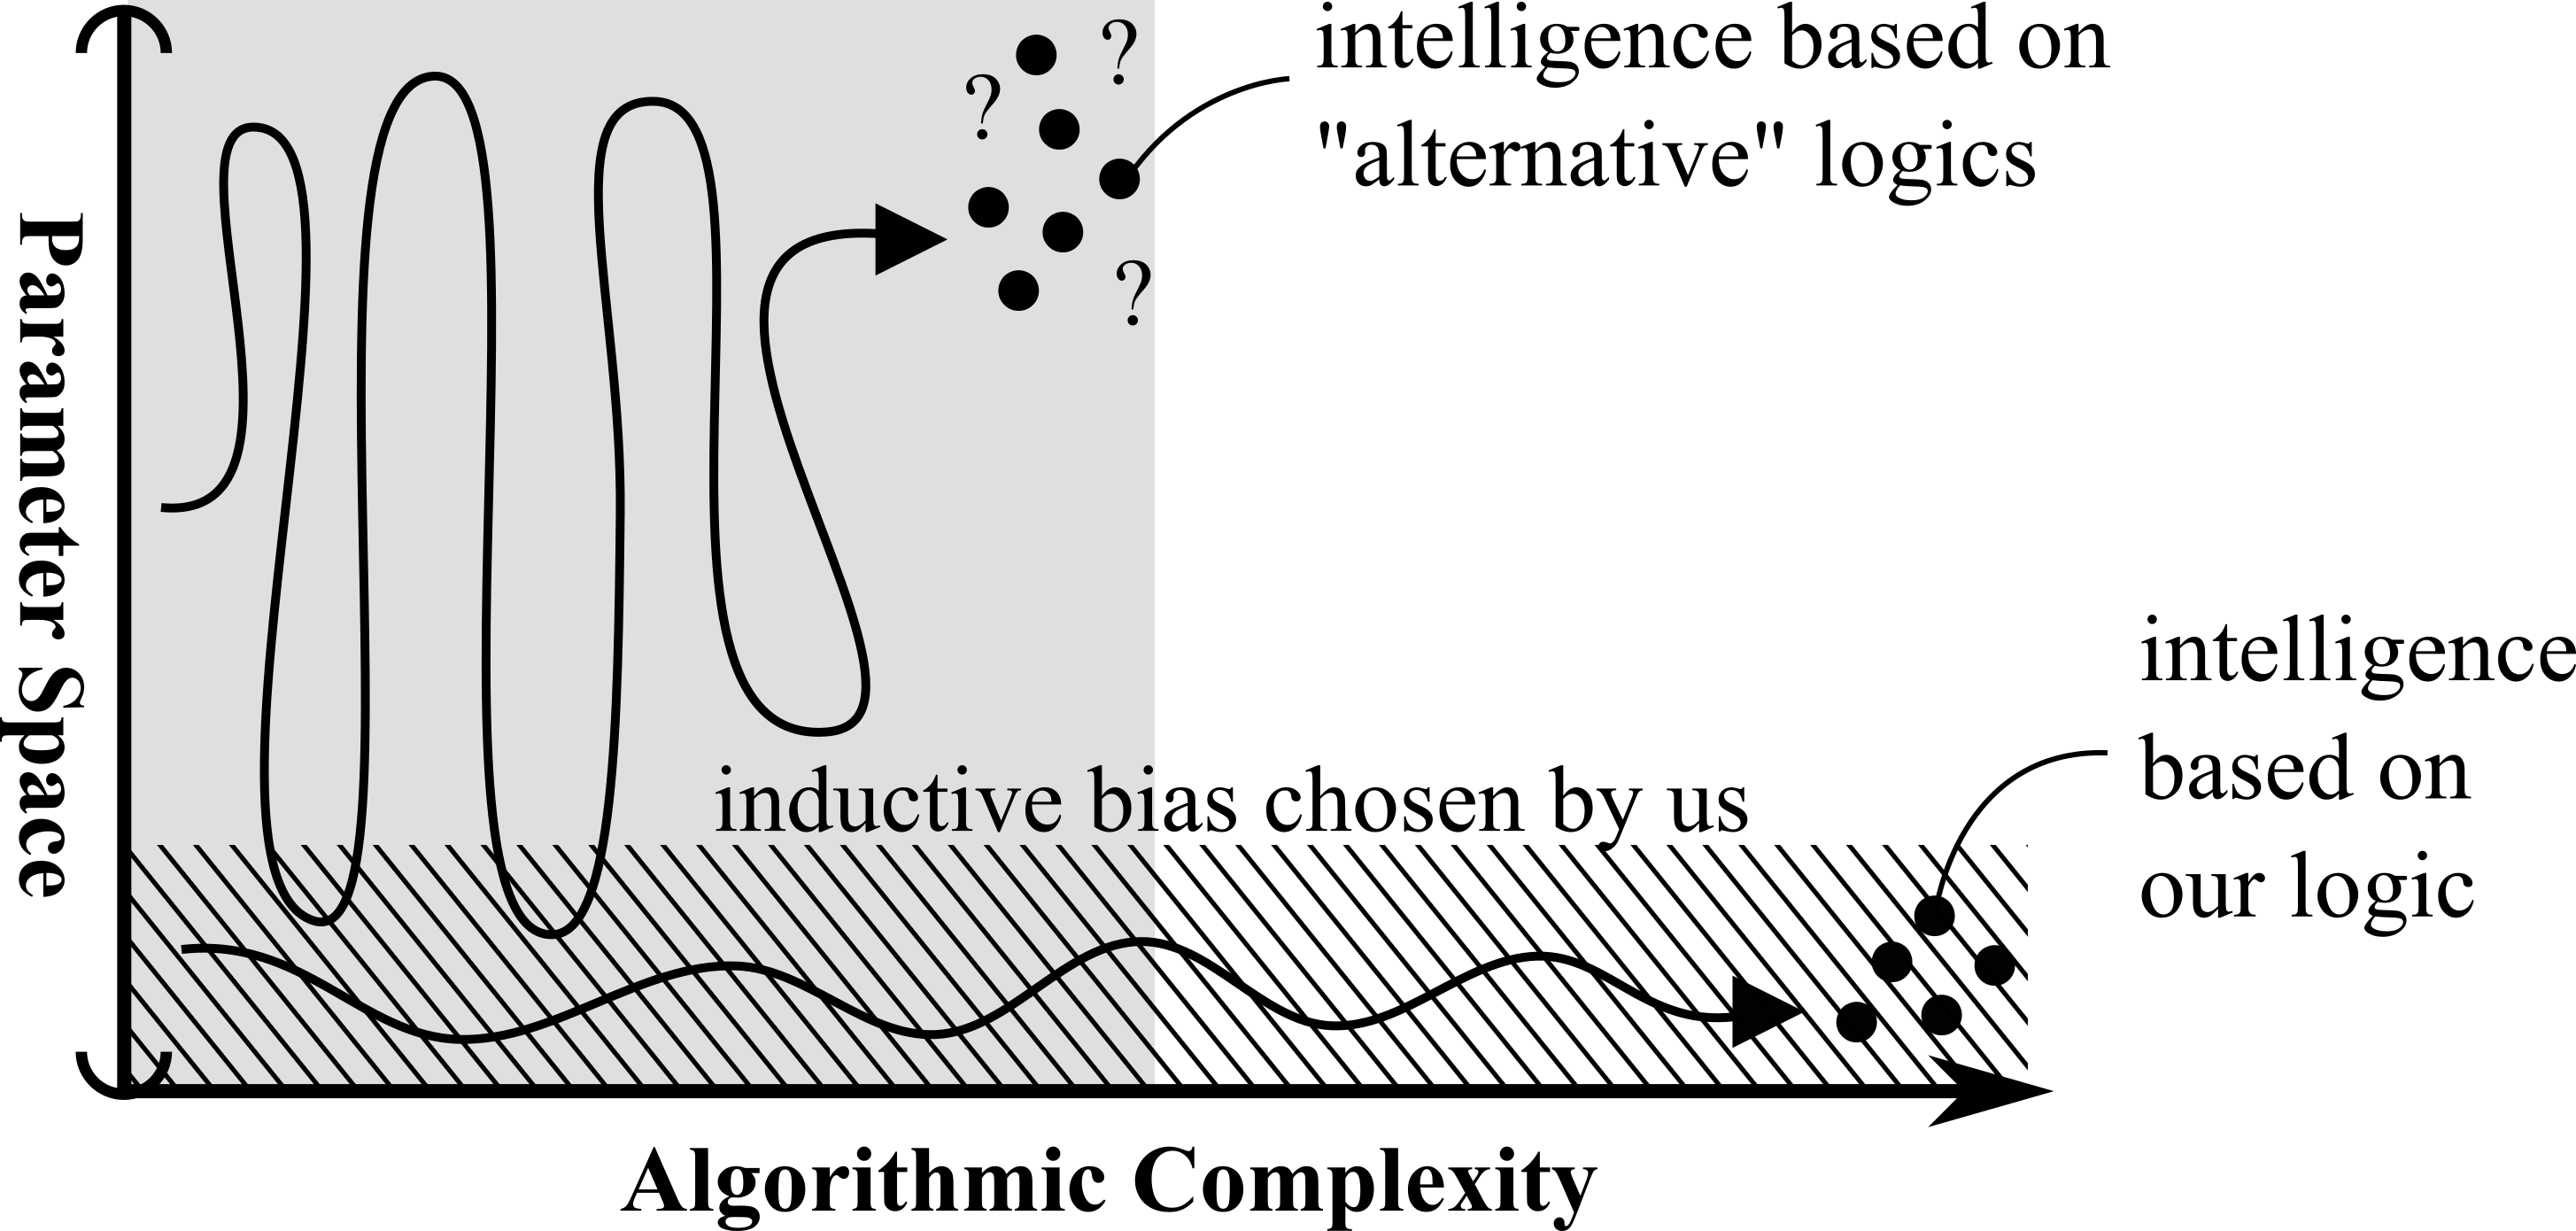
\includegraphics[scale=0.5]{no-free-lunch.png}}}
	\end{equation}
	\item \cc{
	往往如果 归纳偏好 选对了,可以在短时间内找到答案,否则问题是不可解的 (intractable)}{
	Oftentimes, if inductive bias is chosen correctly, solution is found quickly, otherwise problem becomes \textbf{intractable}
	}
\end{itemize}
\end{frame}

\begin{frame}
\frametitle{\cc{Richard Sutton 的观点}{Richard Sutton's view}}
\begin{itemize}
	\item \cc{
	Richard Sutton 认为,我们只需在 强化学习 的框架下 \emp{增加计算力},就可以找到 strong AI}{
	In contrast, Sutton expressed the view that AI can be solved merely by \textbf{increasing computing power}, under the reinforcement learning framework
	}
	\begin{equation}
	\vcenter{\hbox{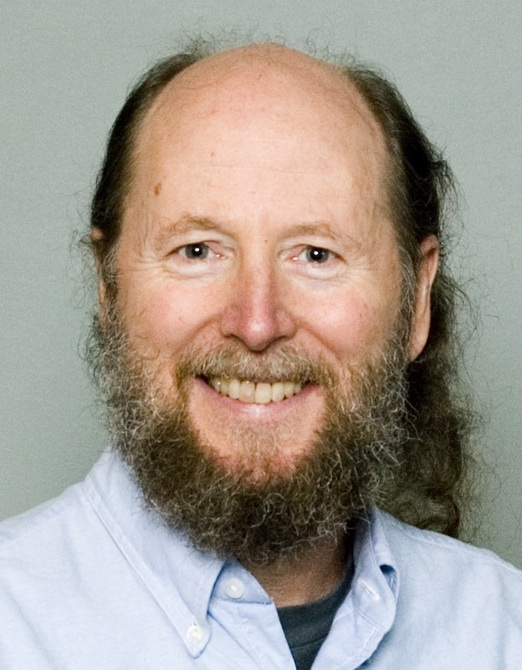
\includegraphics[scale=0.7]{Richard-Sutton.jpg}}}
	\end{equation}
\end{itemize}
\end{frame}

\frameinlbffalse
\begin{frame}
\frametitle{References}
\cc{多谢收看}{Thanks for watching} \smiley \\
% \printbibliography
\end{frame}

\end{document} 